\documentclass[a4paper]{article} % set paper size

\usepackage[utf8]{inputenc}
\usepackage {url}
\usepackage[top=2.0cm, bottom=2.0cm, left=2.54cm, right=2.54cm]{geometry} % set margin
\usepackage{amsfonts} % for set names
\usepackage{amsmath} % for equation system
\usepackage{amsthm} % for theorem block
\usepackage{fixltx2e} % for subscript
\usepackage{fancyhdr} % for footer/headline modification
\usepackage{xcolor}
\usepackage{graphicx,float} % for image insertion
\usepackage{multicol} % for text in tow columns
\usepackage{multirow} % for text in tow columns

\usepackage{wrapfig} % figure wrapping


\pagestyle{fancyplain} % for footing modification on all pages
\fancyhf{}
%\renewcommand{\headrulewidth}{0pt} % remove decorative lign

\fancyhead[L]{Pauline Maury Laribiere\\
              Alexandre Devienne}
\fancyhead[R]{MT/EL-BA2 EPFL \\
                \today}
\fancyhead[C]{\textbf{Spring programming project : Microcosmos}}

\fancyfoot[R]{\thepage\ of \pageref{lastpage}}

\begin{document}
\begin{multicols*}{2}
% =====================================================================
\section{Architecture and implementation details}

\subsection{Architecture}
\begin{figure}[H]
\centering
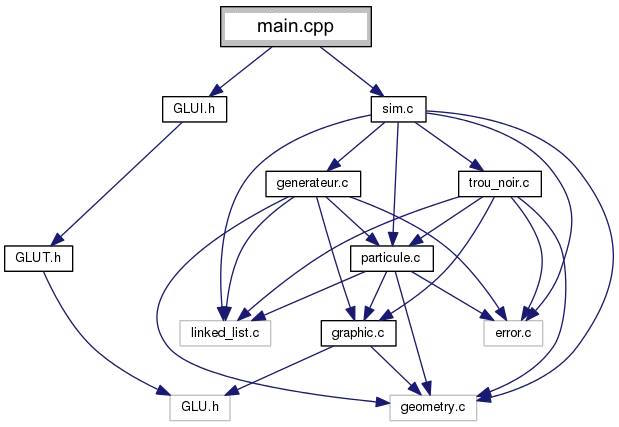
\includegraphics[width=0.48\textwidth]{architecture.jpg}
\caption{Final architecture}
\end{figure}

From \emph{rendu 2} to \emph{rendu 3}, there were not any changes in the
program architecture, we simply finished the code how we had foreseen to do.

The only change to note is that \emph{trou\_noir.c} and \emph{generateur.c} do not rely on \texttt{int part\_closestPartOn(POINT p)}
(as we described in the \emph{rendu }2 report), but on \texttt{bool part\_partsOn(POINT p, LIST\_HEAD linkedList)}.
This small change was needed in \emph{trou\_noir.c} in order to reduce the algorithm complexity.

\subsection{Data management}
To store the data of the simulation's entities (black holes, particles and generators)
we used double linked list (implemented using a generic module).
It was necessary to make sure that all the memory allocated to the program was in use (even after entities deletion).
We considered using arrays, where dichotomy search could have been used, but it would not have reduced the algorithm 'worst-case' complexity.

\subsection{Calculation and memory costs}
Let's study the calculation and memory costs of one step of the simulation.
It is done in 5 parts.

Let $nbP$, $nbTN$ and $nbG$ the number of respectively particles, black holes and generators.
To simplify the calculation, let's consider $nbP$ the number of particles after a step of the simulation.
Indeed, this number could be increased by the creation of particles from generators (to a maximum of $nbG$ more).



\paragraph{Calculation costs}
Using the Big Oh notation, the calculation cost of all steps from the simulation
are summarized in table \ref{tab-calc}. Thus the total complexity of the algorithm is :
\begin{align}
\mathcal{O}(nbP (nbP + nbG + nbTN))
\end{align}


\begin{table}[H]
\begin{center}
\begin{tabular}{|c|c|}
\hline
Step & \multicolumn{1}{|c|}{\multirow{2}{*}{Calculation costs}} \\
subdivision   &  \\
\hline
\hline
Generators &  $nbG\cdot nbP$\\
\hline
Particle  &       \multicolumn{1}{|c|}{\multirow{2}{*}{$nbP$}}\\
initialization &  \\
\hline
Force calculation  & \multicolumn{1}{|c|}{\multirow{2}{*}{$nbTN\cdot nbP$}}\\
(black holes) &  \\
\hline
Force calculation  & \multicolumn{1}{|c|}{\multirow{2}{*}{$nbP^2$}}\\
(particles) &  \\
\hline
Kinematic update  & \multicolumn{1}{|c|}{\multirow{2}{*}{$nbP$}}\\
(particles) &  \\
\hline
Destroying particles &  \multicolumn{1}{|c|}{\multirow{2}{*}{$nbTN\cdot nbP$}}\\
 on black holes &  \\
\hline
\end{tabular}
\end{center}
\caption{Algorithm complexity for a single simulation step}
\label{tab-calc}
\end{table}

\paragraph{Memory costs} All entities data are stored in generic linked lists,
which memory costs are linear in the number of elements thus $nbP + nbG + nbTN$.
In addition to this, in each 5 steps we are not using any recursion and each time we only
declare a few more variables, which number doesn't depend on any amount of entities
with the exception of the last step (destroying particles touching black holes).

For the first 4 steps we have a memory cost of $\mathcal{O}(nbP + nbG + nbTN)$

The last step is a bit more complex :
it creates a linked list of all particles to destroy for every black holes.
So we could think this step is in $\mathcal{O}(nbP \cdot nbTN)$ but since we destroy those particles before
checking the next black holes, we cannot store them in a subsequent linked list.
After a more precise analysis, we see that our algorithm cannot create more than $nbP$ different
elements in the linked list, thus we add $nbP$ to the memory cost of the 4 previous steps
(the black holes data are already accounted for).

Thus the total memory cost is:
\begin{align}
\mathcal{O}(nbP + nbG + nbTN)
\end{align}


\subsection{Illustrations}
See page \pageref{lastpage}
% find nice pictures
% ...

% =====================================================================
\section{Methodology}
\subsection{Work organization}

\paragraph{Workflow.} We used a Git repository (hosted privately on GitHub) from the beginning,
to avoid the hassle of sending code by emails and merging files manually.
It also provided us a great syncing tool, so we could be sure we were working on
the latest version of the code.
Moreover, it forced us to be rigorous in our way to commit our work
because we had to explain every time which changes had been made
(in so called commit messages).

For each \emph{rendu}, we divided the work that had to be done
according to the different testing mode of the program.
For the \emph{rendu 1}, one had to do the Error mode and the other the Force mode.
Then, for \emph{rendu 2}, there were the Graphic and the Integration mode.
Finally, for \emph{rendu 3}, we shared the last specifications:
one finished the OpenGL and GLUT
and the other the remaining part of the Simulation mode.
The person responsible for each module is summarized in table \ref{tab-module}.

This means we only coded once together, but thanks to the Git repository,
we were able to help each other out, easily, efficiently and remotely (which happened often).

\paragraph{Start of the project.} Before even coding a single line, we tried to elaborate the final
architecture we would use. With this (draft of the) architecture done, it was easier
to divide the work between us two.
Then, we began the program with the basics of the particle and geometry module (low level vector calculation).
Then, we worked our way up, from sim to main. Every time, we only wrote the basics of the code so we could begin testing from \texttt{main.cpp}
the function we had coded all the way down.

\paragraph{Testing.}
We mainly compared how our program behaved compared to the specifications and the demo program.
First, with the given testing file, then if a bug arose (or to thoroughly test our code)
we tried with different test files (using a special verbose debug version of our code).
Then if everything looked fine, we could move on to implementing another feature.

To test the generic linked list module, a separate testing environment (outside of the project)
was used, and it proved very useful to iron all the bugs out.

\paragraph{Bugs and issues.}
The most frequent bugs were due to issues with pointers and not initializing variables before using them.

It was also frequent that when testing our code we left some bugs in, which we only found later.
Even if their roots were rapidly found (when we both put our minds into it) it often slowed us.

The bug which took us the longest to solve was the proper drawing of the black holes (dashed lines).
We indeed tried a lot of things, before realizing we only had to change the \texttt{glBegin} parameter from \texttt{GL\_LINE} to \texttt{GL\_LINES}.

% =====================================================================
%\subsection{Person responsible for each module} % change to a table in a floating figure

% =====================================================================
\subsection{Auto-evaluation of our work}
We can say that we are satisfied with our work.
Even though our programming levels were very different,
we both learned a lot thanks to this project.

Now that we gained this experience, we will surely pay more attention to testing our code
before moving on to another feature.
We might also use more advanced Git features (like branches) to have an even better workflow and
avoid some complex merges we had to do.

We did not used the public intermediary \emph{rendu} but it was still a nice asset to have.

A weak point was the fact that the course subjects had to be understood
and used very quickly to succeed in the project.
Also, we were not sure during the exercise sessions if we should focus
on the project or the weekly exercises.

A strong point of the project was its diversity in themes (modeling of particles movement, graphics and user interactions handling)
Also, it was nice to be able to unleash our creativity to create fun and surprising scenarios (see last illustration),
once the project was fully complete (as for \emph{Recolor}).

An improvement might have been a project were we could have started being creative earlier, and not just at the end.

\begin{table}[H]
\begin{center}
\begin{tabular}{|c|c|c|}
\hline
\multicolumn{1}{|c|}{\multirow{2}{*}{Modules}} & Pauline & Alexandre \\
 & Maury Laribière &  Devienne\\
\hline
\hline
\texttt{main.cpp} &  X &\\
\hline
\texttt{sim.c} & &X\\
\hline
\texttt{particule.c} & & X\\
\hline
\texttt{generateur.c} & & X\\
\hline
\texttt{trou\_noir.c} & & X\\
\hline
\texttt{list\_linked.c} & &X\\
\hline
\texttt{geometry.c} & X&\\
\hline
\texttt{graphic.c} & X&\\
\hline
\end{tabular}
\end{center}
\caption{Person responsible for each module}
\label{tab-module}
\end{table}

\section{Conclusion}
This project was challenging to begin, but once the workflow was established, it went smoothly
(if we omit those obscure \texttt{Segmentation fault} along the way).
It was a rewarding experience and we are proud of the result.

\begin{figure}[H]
\centering
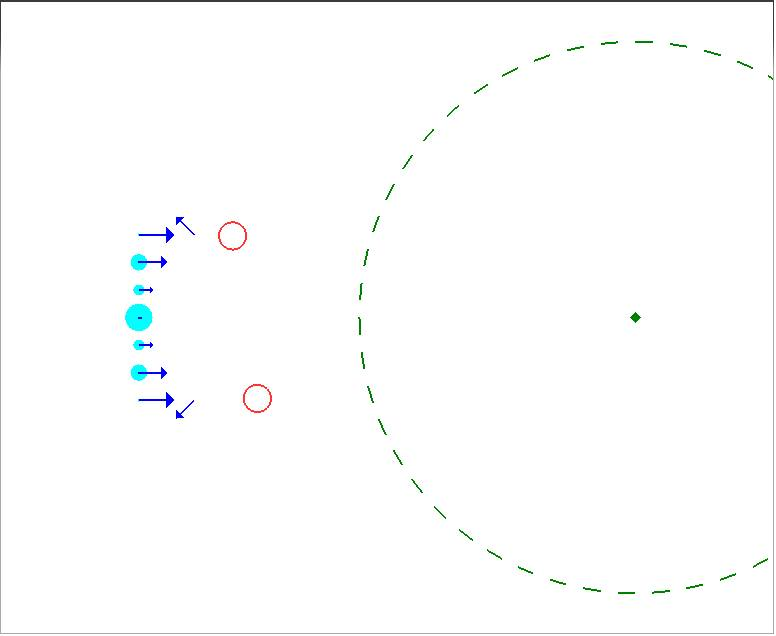
\includegraphics[width=0.48\textwidth]{1.jpg}
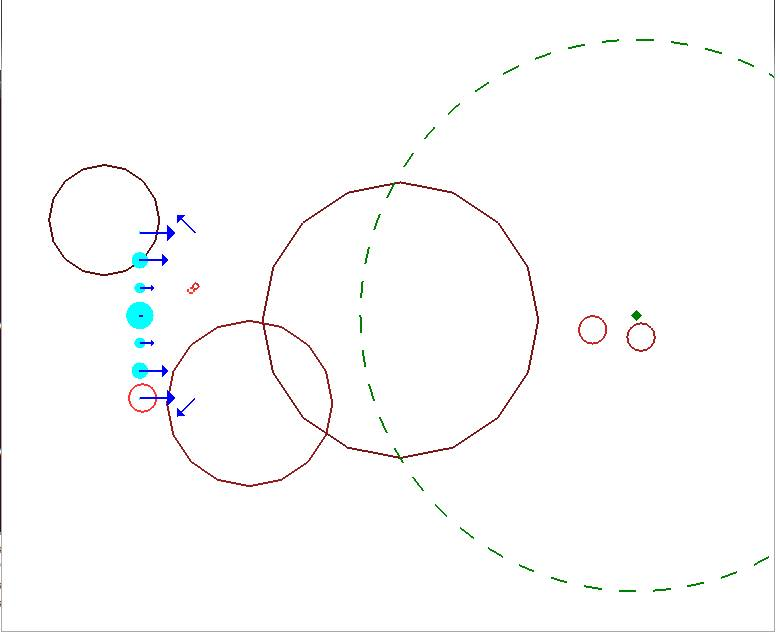
\includegraphics[width=0.48\textwidth]{2.jpg}
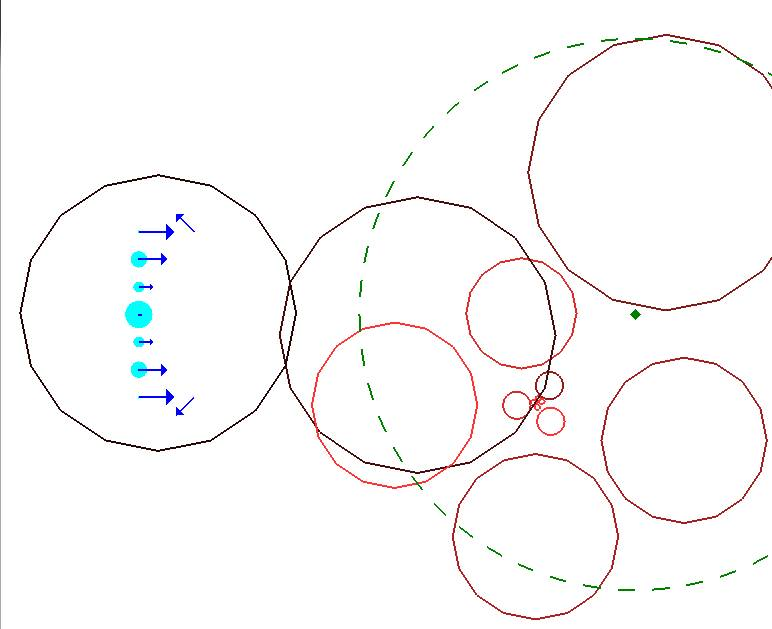
\includegraphics[width=0.48\textwidth]{3.jpg}
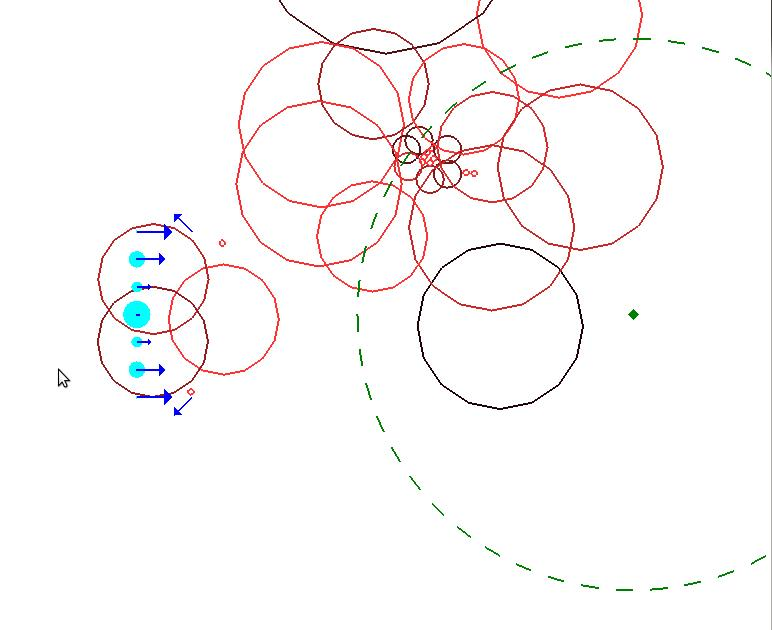
\includegraphics[width=0.48\textwidth]{4.jpg}
\end{figure}
\begin{figure}[H]
\centering
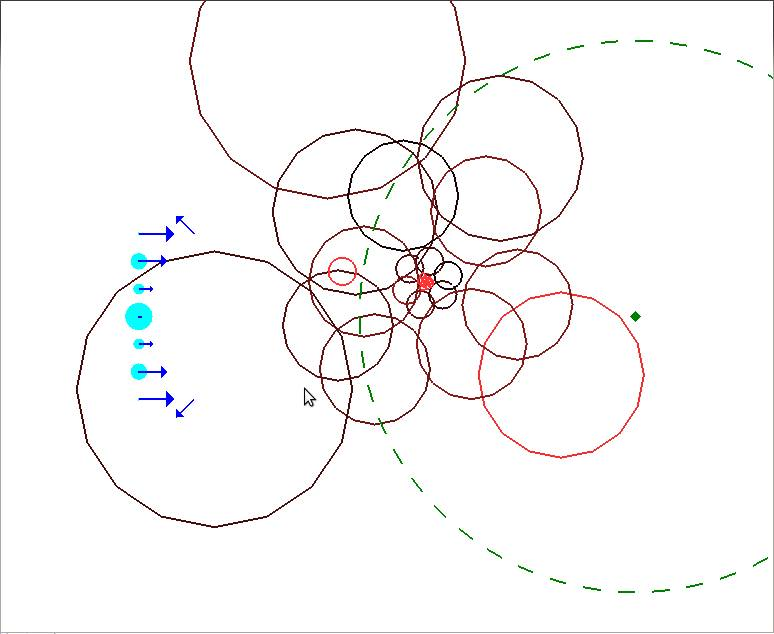
\includegraphics[width=0.48\textwidth]{5.jpg}
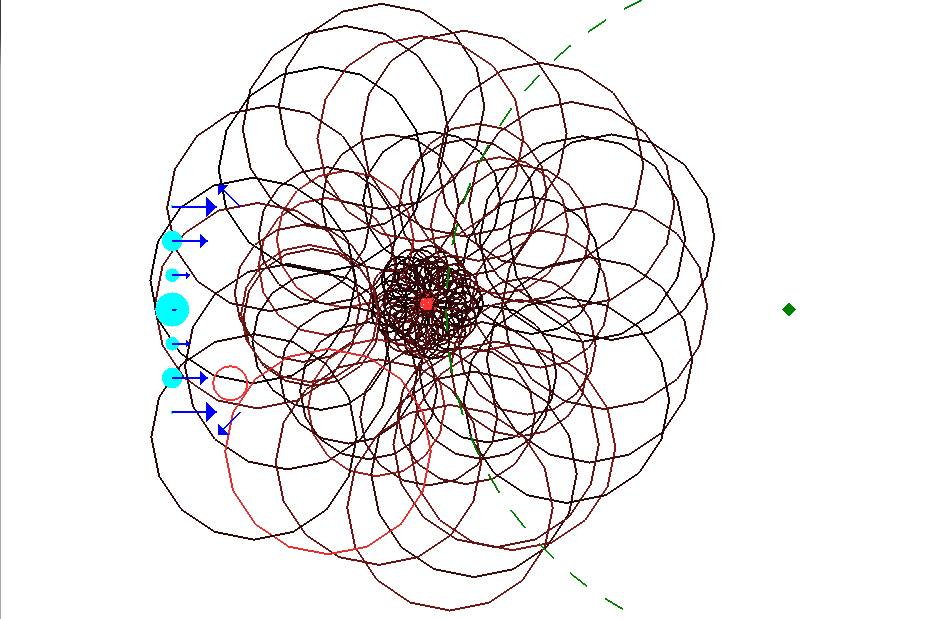
\includegraphics[width=0.48\textwidth]{6.jpg}
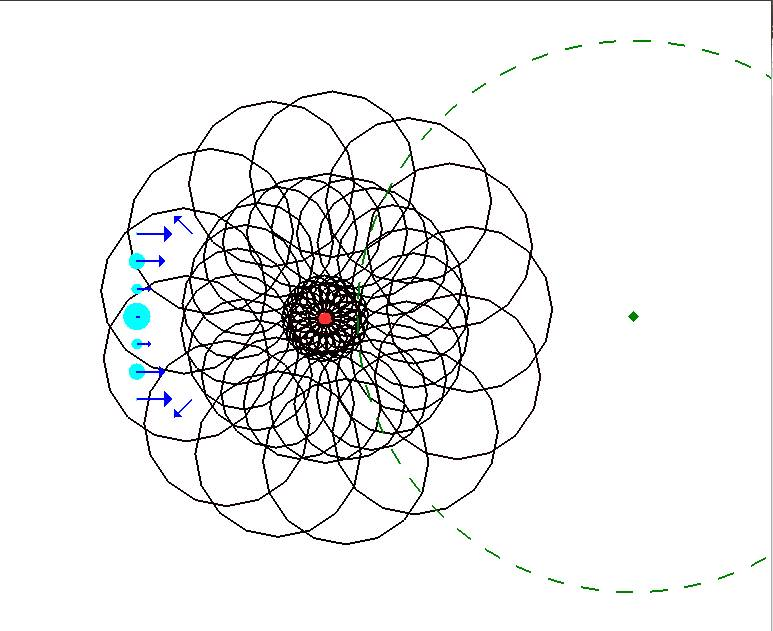
\includegraphics[width=0.48\textwidth]{7.jpg}

\caption{7 images of a single simulation scenario (which begins on the upper left image). In every image there is 9 generators (to the left) and 1 black hole (to the right).
The other circles are particles which total number varies (from the first image to the last) : 2, 8, 14, 30, 30, 127, 96.}
\end{figure}
\label{lastpage}
\end{multicols*}
\end{document}
